\documentclass[a4paper, 12pt]{mcshw}
\DeclareMathOperator*{\argmax}{arg\,max}
\begin{document}
	\Letsmaketitle{1}
    \begin{enumerate}
        \item Project the surface area of a sphere of radius $\sqrt{d}$ in d-dimensions onto a line through the center. For $d$ equal 2 and 3, derive an explicit formula for how the projected surface area changes as we move along the line. For large $d$, argue(intuitively)that the projected surface area should behave like a Gaussian.


            \textbf{Solution:} For any $d$ greater than 1, the projected surface area of a d-dimensional along the line takes non-zero value for $x \in (-\sqrt{d},\sqrt{d})$, has has the formula 
            $$
            {(d - x^2)}^{\frac{d-2}{2}}A(d-1)
            $$
            for $d=2$, the fomula is
            $$
            x=2
            $$
            \begin{center}
                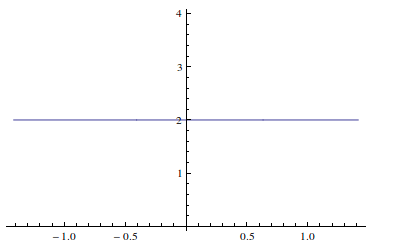
\includegraphics[height=5cm]{1.png}
            \end{center}
            for $d=3$, the fomula is
            $$
            2\pi\sqrt{3 - x^2}
            $$
            \begin{center}
                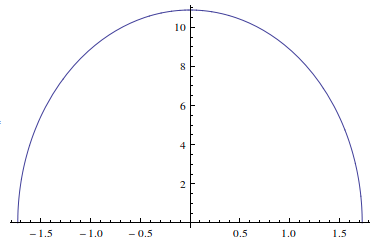
\includegraphics[height=5cm]{2.png}
            \end{center}
            and for large $d$, we observe that
            \begin{align*}
                {(d - x^2)}^{\frac{d-2}{2}}A(d-1)&=A(d-1)(d(1-\frac{x^2}{d}))^{\frac{d-2}{2}}\\
                                                 &=A(d-1)d^{\frac{d-2}{2}}(1-\frac{x^2}{d})^{\frac{d-2}{2}}\\
                                                 &\approx A(d-1)d^{\frac{d-2}{2}}e^{\frac{-x^2}{d}\frac{d-2}{2}}\\
                                                 &\approx A(d-1)d^{\frac{d-2}{2}}e^{\frac{-x^2}{2}}
            \end{align*}
            and it looks like a Gaussian.
            \begin{center}
                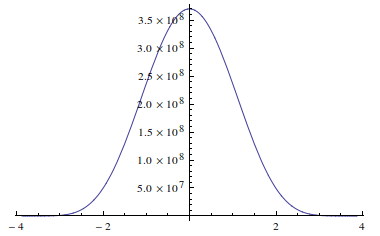
\includegraphics[height=5cm]{3.png}

                \vspace{-6mm}\small{$d=15$}
            \end{center}


        \item For what value of d is the volume, $V(d)$, of a d-dimensional unit sphere maximum? (Hint: Consider the ratio $\frac{V(d)}{V(d-1)}$).


        \textbf{Solution:} First,
        $$
        \frac{V(d)}{V(d-2)}=\frac{(d-2)\sqrt{\pi}\Gamma(\frac{d-2}{2})}{d\Gamma(\frac{d}{2})},\text{for } d\geq1
        $$ 
        for $d=2k, k\geq2$,
        $$
        \frac{V(d)}{V(d-2)}=\frac{(k-1)\pi\Gamma(k-1)}{k\Gamma(k)}=\frac{\pi}{k}
        $$
        then 
        $$
        \argmax_kV(2k)=V(6)=\frac{\pi^3}{6}
        $$
        for $d=2k + 1, k\geq1$,
        $$
        \frac{V(d)}{V(d-2)}=\frac{(2k-1)\pi\Gamma(\frac{2k-1}{2})}{(2k+1)\Gamma(\frac{2k+1}{2})}=\frac{2\pi}{2k+1}
        $$
        then 
        $$
        \argmax_kV(2k+1)=V(5)=\frac{8\pi^2}{15}
        $$
        thus
        $$
        \argmax_dV(d)=\max(V(5), V(6))=V(5)
        $$

    \end{enumerate}
\end{document}
